% Testing Plan Overview
% 01_section.tex
% Author: Sarah Pawlowski 
% Date: 1/12/25

%% begin text
\section{Introduction}
The purpose of this document is to outline the testing procedure for the background noise test
of the ASIO instrument. These tests are meant to establish a baseline background noise level
that will be used as a comparison for future tests run on the instrument, refer to the ASIO
MSU Testing Overview (BUBO-TEST-0012) for descriptions of these tests. Additionally, these
tests are a first indicator if the housing of ASIO is light-tight before completing more rigorous
and specific light-tightness tests. An ESD safe smock, grounding bracelet and grounding strap
should be worn while handling ASIO.

\subsection{Required Testing Equipment}
\begin{table}[h!]
	\centering \caption{Testing Equipment}
	\begin{tabular}{|c|}
		\hline
		\textbf{Required Equipment} \\
		\hline
	ASIO Instrument \\
        External Computer \\
        Ground Support Software \\
        Cables \\
        Keysight E36313A Bench Power Supply \\
        RS422 to USB converter \\
        11 -  Thorlabs SM1CP2 end caps \\
        Dark Box \\
        ESD safety Equipment \\
        \hline
	\end{tabular}
\end{table}

\subsection{Test Engineer(s)}
\begin{table}[H]
	\centering
	\begin{tabular}{p{2in} p{2in} p{2in}}
		& & \\
		& & \\ \hline
		Test engineer & Signature & Date \\
		& & \\
		& & \\ \hline
            Test engineer & Signature & Date \\
            & & \\
		& & \\ \hline
            Test engineer & Signature & Date \\
	\end{tabular}
\end{table}

\subsection{Instrument Description}
The diagrams below show the the connectors and the front face of the ASIO instrument. See the ICD (BUBO-SYSE-0001) for the full pinout details of each connector and more details on how to interface with each connector correctly.

\begin{figure}[H] 
    \centering
    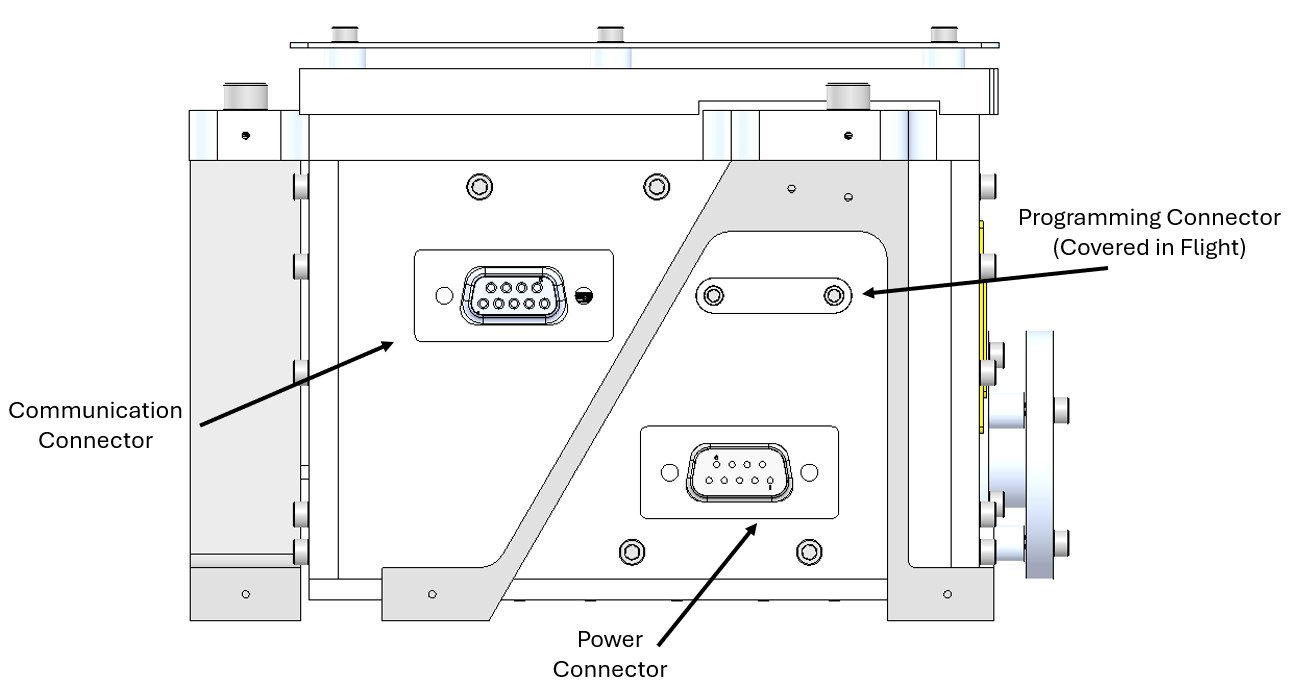
\includegraphics[width=6in]{images/BUBO - connector interface.jpg}
    \caption[ASIO Connector Interface], {ASIO Connector Interface when ASIO is mounted on the optical bench for testing the vent is facing down towards the bench. This makes the communication connector the port above the power connector.}
    \label{fig:ASIO Connector Interface}
\end{figure}

The detectors are numbered as shown in figure \ref{fig:LabeledDetectors} below. These background noise tests are conducted on the ASIO instrument as a whole, rather than individual photodiodes or channels. This figure is for reference only and will not be used to label datasets.

\begin{figure}[H] 
    \centering
    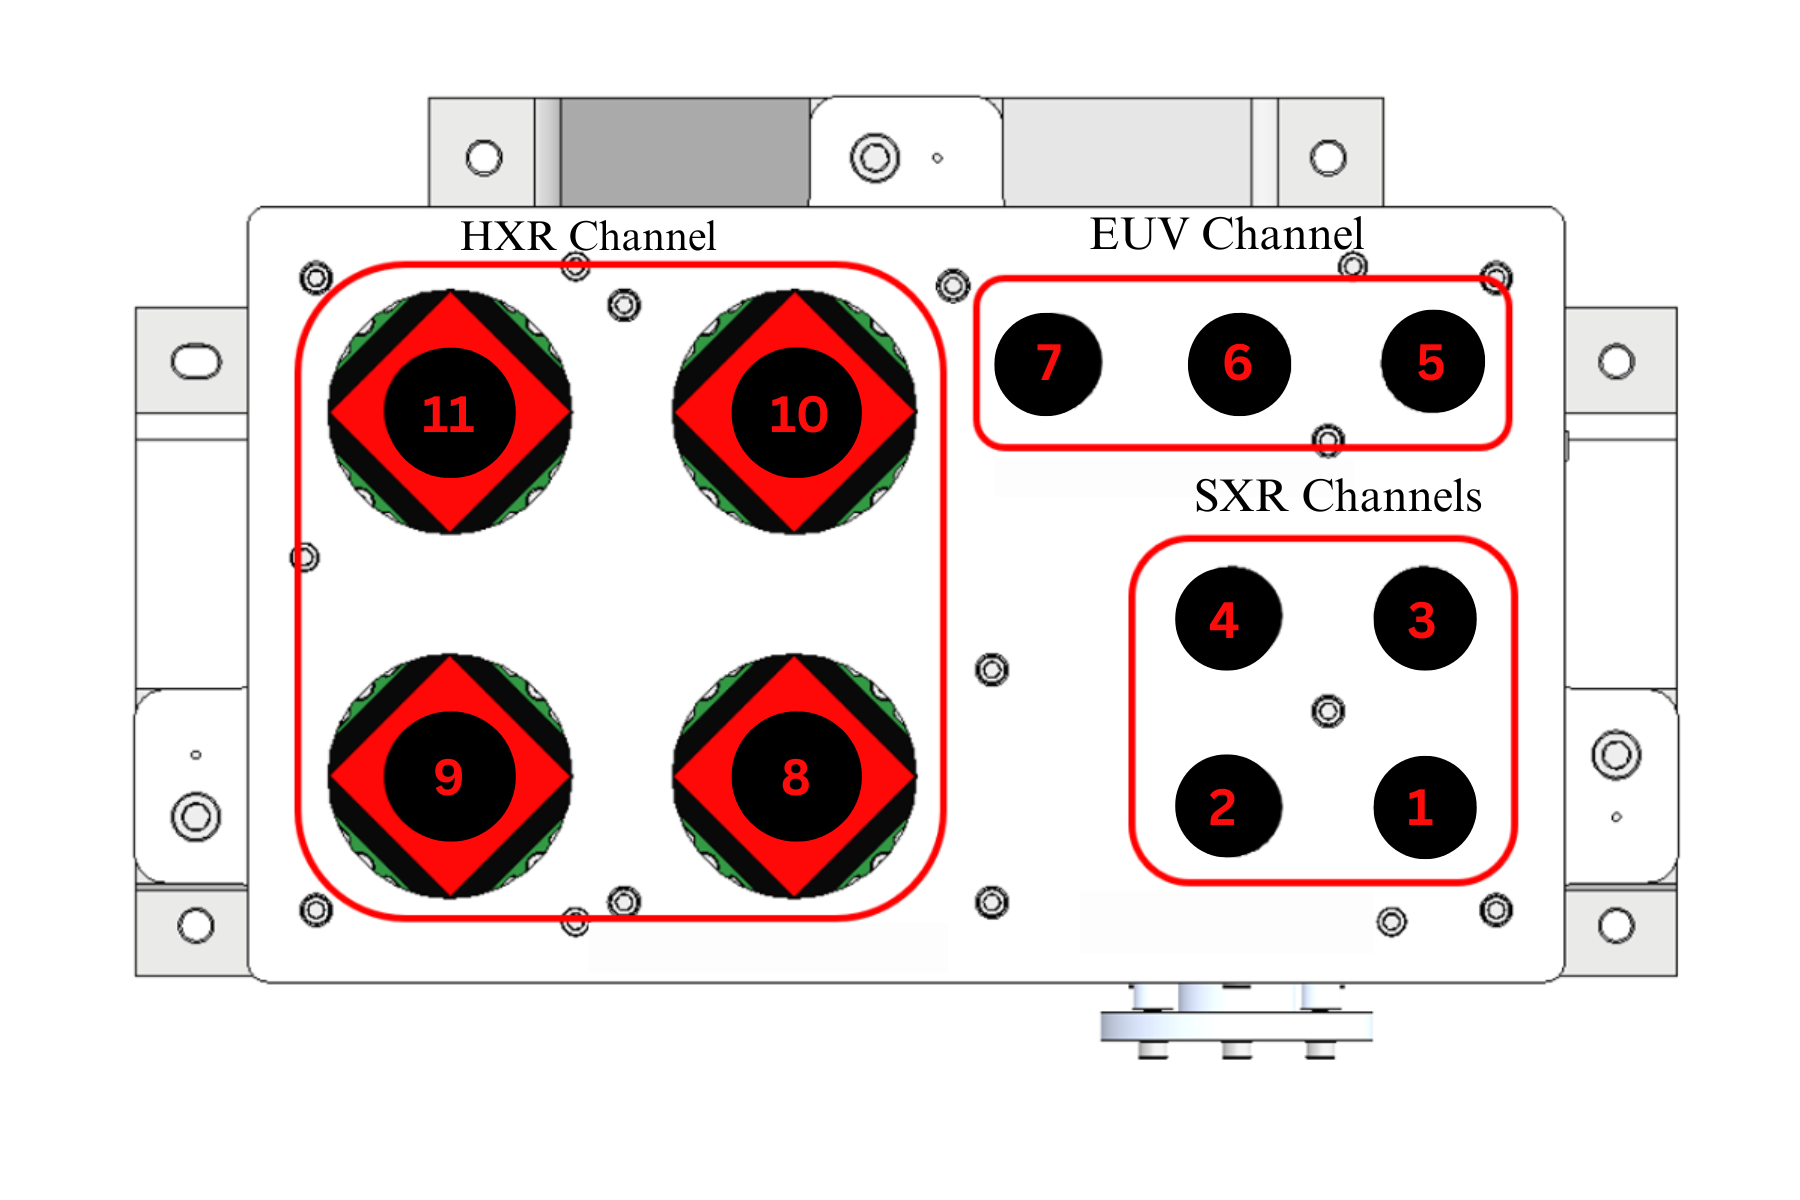
\includegraphics[width=6.5 in]{images/Photodiode_Diagram.png}
    \caption[ASIO Detector Labels]{ASIO Detector Labels, oriented in the same direction instrument is connected to optical bench.}
    \label{fig:LabeledDetectors}
\end{figure}

